\documentclass{ieeeaccess}
\usepackage{cite}
\usepackage{amsmath,amssymb,amsfonts}
\usepackage{algorithm}
\usepackage{algorithmicx}
\usepackage{algpseudocode}
%% \usepackage{caption}
\usepackage{graphicx}
\usepackage{textcomp}

\usepackage{bm}

\usepackage{multirow}

% \usepackage{hyperref}

\usepackage{array}
\setlength\extrarowheight{3pt}

\algnewcommand\algorithmicforeach{\textbf{for each}}
\algdef{S}[FOR]{ForEach}[1]{\algorithmicforeach\ #1\ \algorithmicdo}

\providecommand{\e}[1]{\ensuremath{\times 10^{#1}}}

\def\BibTeX{{\rm B\kern-.05em{\sc i\kern-.025em b}\kern-.08em
    T\kern-.1667em\lower.7ex\hbox{E}\kern-.125emX}}
\begin{document}
\history{Date of publication xxxx 00, 0000, date of current version xxxx 00, 0000.}
\doi{10.1109/ACCESS.2017.DOI}

\title{Using Fuzzy Inference Systems for the Creation of Forex Market Predictive Models}
\title{}
\author{
    \uppercase{Amaury Hernandez-Águila\authorrefmark{1},
    \uppercase{Mario García-Valdez\authorrefmark{1}
      and
    Juan-Julián Merelo-Guervós\authorrefmark{2}}}}
\address[1]{National Technological Institute of Mexico, Calzada Del Tecnológico s/n, Fraccionamiento Tomas Aquino, Tijuana, BC 22414 Mexico (e-mail: {amerhag,mario}@tectijuana.edu.mx)}
\address[2]{University of Granada, Campus Aynadamar Daniel Saucedo Aranda s/n, Granada 18071, 80523 Spain (e-mail: jmerelo@geneura.ugr.es)}
% Grant information.
% TODO 1:
\tfootnote{This paragraph of the first footnote will contain support 
information, including sponsor and financial support acknowledgment. For 
example, ``This work was supported in part by the U.S. Department of 
Commerce under Grant BS123456.''}

\markboth
{Author \headeretal: Preparation of Papers for IEEE TRANSACTIONS and JOURNALS}
{Author \headeretal: Preparation of Papers for IEEE TRANSACTIONS and JOURNALS}
% Do we need to change this?
% TODO 2: 

\corresp{Corresponding author: Mario García-Valdez (e-mail: mario@tectijuana.edu.mx).}

% You must justify why do we care, in the beginning, 
% Why is this problem important?
% Why is this solution needed?
% Why is it better?
% Amaury: I state that the method is competitive. I don't want to
% Amaury: say that it is better because it is interpretable or anything
% Amaury: like that, because I didn't perform experiments to prove that.
% All this is very brief just a short sentence for each - Mario
% We will try not to use a Passive voice when we can - Mario
% TODO 3: COMPLETE.

\begin{abstract}

\end{abstract}

\begin{keywords}
% TODO 6: COMPLETE. I added some of the keywords from Munkhdalai2019.
% I'm already using kewords from
% http://www.ieee.org/organizations/pubs/ani_prod/keywrd98.txt
  Economic forecasting, fuzzy systems, multi-agent system, activation function, forex market.
\end{keywords}

\titlepgskip=-15pt

\maketitle

\section{Introduction}
\label{section:introduction}

\section{Preliminaries}
\label{section:preliminaries}

\section{Proposed Method}
\label{section:proposed-method}

\section{Implementation}
\label{section:implementation}

\section{Experiments}
\label{section:experiments}

\section{Results}
\label{section:results}

\section{Conclusion}
\label{section:conclusion}

\section{Future Work}
\label{section:future-work}

\section*{Acknowledgment}

\begin{IEEEbiography}[{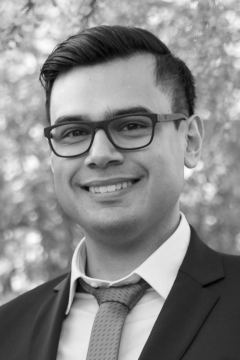
\includegraphics[width=1in,height=1.25in,clip,keepaspectratio]{img/amaury-1by1half-in.png}}]{Amaury
  Hernandez-Aguila} 
\end{IEEEbiography}

\bibliography{bibliography}
\bibliographystyle{IEEEtran}

\EOD

\end{document}
